%-----------------------------------------------------------------------------
%
%               Template for LaTeX Class/Style File
%
% Name:         sigplanconf-template.tex
% Purpose:      A template for sigplanconf.cls, which is a LaTeX 2e class
%               file for SIGPLAN conference proceedings.
%
% Author:       Suresh Thummalapenta
%               Department of Computer Science
%								North Carolina State University, Raleigh, USA
%               sthumma@ncsu.edu
%
% Created:      08 August 2007
%
%-----------------------------------------------------------------------------


\documentclass{sigplanconf}

\usepackage{amsmath}
\usepackage{cite}
\usepackage{url}
\usepackage{alltt}
\usepackage{graphicx}

%-- User defined macros ---
\newcommand{\CodeIn}[1]{{\small\texttt{#1}}}
\newcommand{\Comment}[1]{}
\newcommand{\Fix}[1]{{\large\textbf{FIX}}#1{\large\textbf{FIX}}}
\newenvironment{CodeOut}{\begin{small}}{\end{small}}
\newenvironment{SmallOut}{\begin{small}}{\end{small}}

\begin{document}

\authorpermission
\conferenceinfo{OOPSLA'07,} {October 21--25, 2007, Montr{\'e}al, Qu{\'e}bec, Canada.}
\CopyrightYear{2007}
\copyrightdata{978-1-59593-786-5/07/0010} 

%\titlebanner{banner above paper title}        % These are ignored unless
%\preprintfooter{short description of paper}   % 'preprint' option specified.

\title{Exploiting Code Search Engines to Improve Programmer Productivity}

\authorinfo{Suresh Thummalapenta}
           {Department of Computer Science, North Carolina State University\\Raleigh, NC 27695, USA}
           {sthumma@ncsu.edu}

\maketitle

\begin{abstract}
Code Search Engines (CSE) can serve as powerful resources of open
source code, as they can search in billions of lines of open source
code available on the web. The strength of CSEs can be used for
several tasks like searching relevant code samples, identifying
hotspots, and finding bugs. However, the major limitations in using
CSEs for these tasks are that the returned samples are too many and
they are often partial. Our framework addresses the preceding
limitations and thereby helps in using CSEs for these tasks. We
showed the effectiveness of our framework with two tools developed
based on our framework.
\end{abstract}

\category{D.2.3}{Software Engineering}{Coding Tools and Techniques}[Object-oriented programming]
\terms 
Languages, Experimentation.
\keywords
Code reuse, Code search engine, Code examples, hotspots.

\section{Introduction}
Various Code Search Engines (CSEs)\footnote{\url{http://gonzui.sourceforge.net/links.html}}
are available on the web that can search in billions of lines of available open source code. 
\Comment{Some of these CSEs like Google, Koders, DocJar, Codease, and Krugle are non-academic. SPARS-J and 
Sourcerer are two of the few academic code search engines.} Given a query, CSEs 
can suggest relevant code samples with usages of keywords in the given query. But these CSEs
are not quite helpful in practice, as they often produce a large number of code
examples for a given query and the desired code sample is often not available 
among the first several results. For example, the Google Code Search Engine
(GCSE)\footnote{\url{http://www.google.com/codesearch}} 
returns near 5000 samples for the query \CodeIn{lang:java
java.sql.Statement executeUpdate}.\Comment{; this query can be used to
extract information regarding the usage of Application Programming Interface (API) 
\CodeIn{executeUpdate} of \CodeIn{java.sql.Statement} class of JDBC.}

Along with assisting programmers in reusing code samples
from existing frameworks or libraries, the code samples 
returned by CSEs can also be used for other tasks 
like identifying framework hotspots and finding bugs in projects 
that reuse open source frameworks or libraries. 
Exploiting CSEs for these tasks requires analysis of 
code samples returned by CSEs. This analysis of code samples 
is non-trivial because the code samples returned by CSEs are often partial. 
The reason for partial code samples is that CSEs retrieve 
only source files with usages of the given query instead of entire projects. 
Due to the preceding limitations, traditional code analysis cannot be applied 
for analyzing the gathered code samples. Therefore, our framework 
uses several heuristics (Section ~\ref{sec:framework}) 
for analyzing these code samples and transforms them into 
an intermediate form. We used the Directed Acyclic Graph
(DAG) as an intermediate form because the DAG represents control-flow information
through its branches and joins, and provides effective traversal mechanisms. 

We developed two tools by extending our framework: PARSEWeb
and Hotspotter. We showed the effectiveness of our framework by comparing the results 
of developed tools with the results of related tools.

\section{Framework}
\label{sec:framework}

Our framework consists of three major components: the code downloader,
code search engine, and code analyzer. Figure~\ref{fig:architecture}
shows an overview of all components and flows among different components.

\begin{figure}[t]
\centering
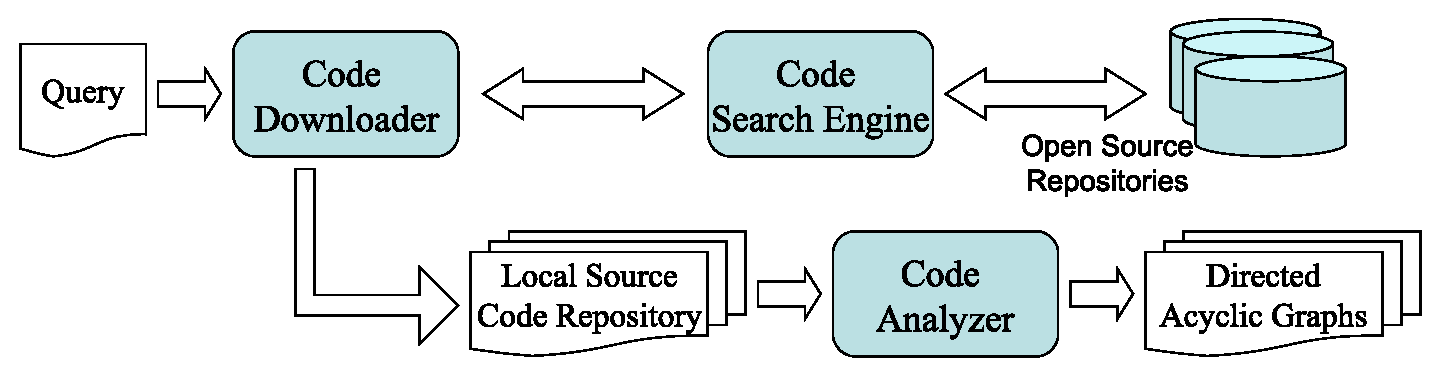
\includegraphics[scale=0.34,clip]{Framework1.eps}
\caption{Overview of the framework} \label{fig:architecture}
\vspace*{-1ex}
\end{figure}

Given a query, the code downloader interacts with a CSE and downloads
relevant code samples. The downloaded code samples, which are partial, form a local
source code repository that serves as input to the code analyzer.
The code analyzer performs static analysis over each code sample with heuristics and
transforms the sample into an intermediate form represented as a DAG.
During transformation, statements inside loops like \emph{while} and \emph{for}
are treated as a group of statements that are executed either once or not.
While constructing DAG, the code analyzer also performs method inlining
by replacing method invocations of the current class with the
body of the corresponding method declarations. Each node in the constructed
DAG represents a statement in the code sample. During transformation,
the code analyzer uses several heuristics to gather additional type information
for each statement. For example, the additional type information for
a method-invocation statement includes the receiver object type, the
return object type, and argument types. We explain a heuristic
used in our framework through the code sample shown below:

\begin{CodeOut}
\begin{alltt}
\textbf{public} QueueSession test()\hspace*{0.2in}\{ ...
\hspace*{0.4in}\textbf{return} connect.createQueueSession(false,int);\}
\end{alltt}
\end{CodeOut}
\vspace*{-1ex}

In this code sample, the method-invocation
\CodeIn{createQueueSession} is a part of the return statement. The
receiver object type of method-invocation
\CodeIn{createQueueSession} can be inferred by looking up the
declaration of the \CodeIn{connect} variable. But as our framework
deals with the code sample that is partial, it is difficult to get
the return type of the method-invocation with out being able to
access the corresponding method declaration in the downloaded file.
However, the return type can still be inferred from the return type
of the enclosing method declaration. As the enclosing method
declaration has return type \CodeIn{QueueSession}, we can infer that
the return type of the method-invocation \CodeIn{createQueueSession}
is \CodeIn{QueueSession} or one of its subtypes. In our framework
implementation, we used GCSE as an underlying CSE.
%-------------------------------------------------------------------------------
\section{Tools}
\label{sec:extensions}

We developed two tools by extending our described framework. The results of these tools
show the effectiveness of our framework.
\Comment{PARSEWeb takes queries of the form ``\emph{Source Object Type} $\rightarrow$
\emph{Destination Object Type}'' as input and suggests frequent method-invocation
sequences that can take the \emph{Source Object Type} as input
and result in the \emph{Destination Object Type}. The second tool, called Hotspotter,
extends the described framework for identifying usage hotspots and weakspots in the library or framework given as input.}
%-------------------------------------------------------------------------------
\subsection{PARSEWeb}
\label{sec:parseweb}

\begin{figure}[t]
\centering
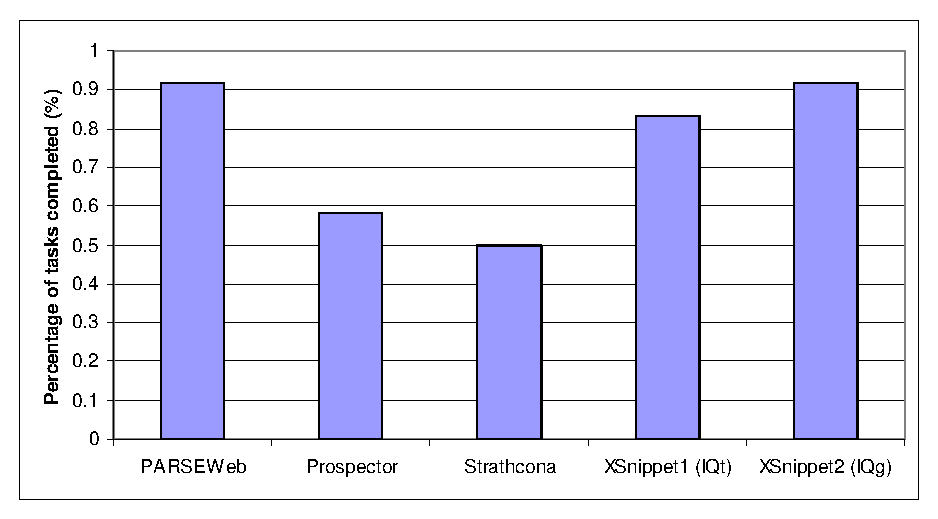
\includegraphics[scale=0.48,clip]{ComparisonResults1.eps}
\caption{Evaluation results of PARSEWeb with related tools Prospector, Strathcona, and XSnippet} \label{fig:comparison}
\vspace*{-2ex}
\end{figure}
A common problem faced by programmers while reusing existing
frameworks or libraries is that the programmers often know what type
of object that they need, but do not know how to get that object
with a specific method sequence. We developed PARSEWeb to address
the preceding issue. PARSEWeb\footnote{Available at
\url{http://ase.csc.ncsu.edu/parseweb/}} accepts a query of the form
``\emph{Source} $\rightarrow$ \emph{Destination}'', and gives the
\emph{Source} and \emph{Destination} object types as input to the
described framework, which in turn provides graphs (DAG) for each
downloaded code sample as output. PARSEWeb identifies nodes that
contain the given \emph{Source} and \emph{Destination} object types
as Source and Destination nodes, respectively. PARSEWeb extracts a
method-invocation sequence by calculating the shortest path between
Source and Destination nodes. We evaluated PARSEWeb with related
existing tools Prospector~\cite{prospector:jungloid},
Strathcona~\cite{strathcona:se}, and XSnippet~\cite{xsnippet:saha}
for 12 specific programming tasks taken from the XSnippet approach.
The results of our evaluation are shown in
Figure~\ref{fig:comparison}. The XSnippet1 and XSnippet2 entries
show results with two query-type techniques $IQ_{T}$ and $IQ_{G}$ of
XSnippet, respectively. PARSEWeb performed better than Prospector,
Strathcona, and XSnippet1. The results of PARSEWeb are at par with
XSnippet2. Moreover, as PARSEWeb is developed based on our framework
that uses CSEs for gathering relevant code samples on demand, unlike
other related tools, PARSEWeb is not limited to the queries of any
specific set of frameworks or libraries. \Comment{The results
signify the effectiveness of the underlying framework used by
PARSEWeb. $IQ_{G}$ query type (XSnippet2). However, the
``XSnippet2'' cannot effectively address the issue targeted by
PARSEWeb as this query type simply returns the set of all code
samples contained in the sample repository that instantiate the
given \emph{Destination} object type, irrespective of the
\emph{Source} object type.}

%-------------------------------------------------------------------------------
\subsection{Hotspotter}
\label{sec:hotspotter}

\setlength{\tabcolsep}{1pt}
\begin{table}[t]
\begin{SmallOut}
\begin{CodeOut}
\begin{center}
\begin {tabular} {|c|l|c|c|c|c|c|c|c|}
\hline
S.No.&Subject&Total&\multicolumn{2}{|c|}{Hotspots}&\multicolumn{2}{|c|}{Weakspots}&\multicolumn{2}{|c|}{Deadspots}\\
\cline{4-9}
&Name&No. of APIs&No.&\%&No.&\%&No.&\%\\
\hline 1&JUnit&379&22&5.8&83&21.9&124&32.7\\
\hline 2&Log4j&1334&21&1.6&180&13.5&746&55.9\\
\hline 3&BCEL&2691&18&0.7&486&18.1&1867&69.4\\
\hline 4&Struts&4679&28&0.6&0&0&4332&92.6\\
\hline
\end{tabular}
\centering \caption {\label{tab:hotspotterresults} Evaluation results
 of Hotspotter with four subjects}
\centering {\CodeIn{Total: Total number of APIs, No.: Number of APIs identified as hotspots, weakspots, and deadspots
and their percentage (shown with \%) among the total number of APIs.}}
\end{center}
\end{CodeOut}
\end{SmallOut}
\vspace*{-4ex}
\end{table}
Object-oriented frameworks are designed mainly with the concern of
reusability. Framework users, who develop concrete applications by
customizing frameworks, must be aware of its areas of flexibility
that are commonly referred as hotspots. We developed Hotspotter for
identifying hotspots in a given input framework. These hotspots can
serve as a starting point for users of the input framework.
Hotspotter also assists framework developers by identifying
weakspots and deadspots. Weakspots are APIs that are rarely used and
deadspots are APIs that are not used among the samples gathered from
CSEs. These weakspots and deadspots can help developers to analyze
whether to keep those APIs in further versions or whether the
functionality provided by those APIs is subsumed by other APIs.

Hotspotter identifies hotspots, weakspots, and deadspots in the given input framework by
calculating the Usage Percentage (\emph{UP}) of each public or protected API among
the code samples returned by the CSE. The \emph{UP} of an API is calculated as
(\CodeIn{No. of usages of the API} / \CodeIn{Total no. of usages of all APIs}) * 100.
Hotspotter uses two threshold values: Upper Threshold (\emph{UTH}) and Lower Threshold (\emph{LTH}).
APIs with \emph{UP} more than \emph{UTH} are classified
as hotspots and APIs with \emph{UP} less than \emph{LTH} and greater than zero are classified as weakspots.
APIs with \emph{UP} of zero are classified as deadspots.
In our implementation, we used \emph{UTH} value as 1\% and \emph{LTH} value as 0.1\%.
We plan to find optimum values for these parameters by
analyzing other open source frameworks. Table~\ref{tab:hotspotterresults} shows
preliminary results of Hotspotter with four subject frameworks JUnit, Log4j,
BCEL, and Struts. Our results show that the framework users often use only a small subset of the
total number of APIs provided by the framework.

%-------------------------------------------------------------------------------
\section{Conclusion}
\label{sec:conclusion}

To exploit code search engines for several tasks that can help
improve the productivity of programmers, we developed an extensible
framework that helps to use the strength of code search engines and
addresses the major limitations in using CSEs for those tasks. Our
framework includes several heuristics to deal with partial code
samples returned by CSEs. We showed the effectiveness of our
framework with two tools developed based on our framework. In future
work, we plan to extend our framework for detecting bugs by mining
specification patterns from the code samples returned by CSEs. As
the current implementation is dependent on the code samples gathered
through GCSE, we plan to extend our framework to collect samples
from other CSEs like Krugle and Koders to analyze results across
different CSEs.

\begin{thebibliography}{1}

\bibitem{strathcona:se}
R.~Holmes and G.~Murphy.
\newblock Using structural context to recommend source code examples.
\newblock In {\em Proc. of ICSE}, pages 117--125, 2005.

\bibitem{prospector:jungloid}
D.~Mandelin, L.~Xu, R.~Bodik, and D.~Kimelman.
\newblock Jungloid mining: helping to navigate the api jungle.
\newblock In {\em Proc. of PLDI}, pages 48--61, 2005.

\bibitem{xsnippet:saha}
N.~Sahavechaphan and K.~Claypool.
\newblock {X}{S}nippet: {M}ining {F}or {S}ample {C}ode.
\newblock In {\em Proc. of OOPSLA}, pages 413--430, 2006.

\end{thebibliography}

\end{document}
1-59593-090-6/05/0007